\documentclass[a4paper]{article}
\usepackage[utf8]{inputenc}
\usepackage[a4paper, total={6in, 8in}]{geometry}
\usepackage[english]{babel}
\usepackage{graphicx}
\usepackage[export]{adjustbox}
\usepackage{subcaption}
\usepackage{wrapfig}
\usepackage{array}
\usepackage{multirow}
\usepackage{makecell}
\usepackage{hhline}
\usepackage{lipsum}
\usepackage[pdftex,dvipsnames,table]{xcolor}
\usepackage{xcolor}
\usepackage{graphicx}
\usepackage{float}
\usepackage{longtable}
\usepackage[bottom]{footmisc}
\usepackage{hyperref}

% Itemize
\usepackage{enumitem}
\setlist[1]{itemsep=0pt}

% code package
\usepackage{listings}

% comment package
\usepackage{comment}

% ToDo package and config
\usepackage{xargs}
\usepackage[colorinlistoftodos,prependcaption,textsize=tiny]{todonotes}
\newcommandx{\mytodo}[2][1=]{\todo[linecolor=red,backgroundcolor=red!25,bordercolor=red,#1]{#2}}
\usepackage{marginnote}
\renewcommand{\marginpar}{\marginnote}

% VU colors
\definecolor{vu-black}{HTML}{000000}
\definecolor{vu-white}{HTML}{ffffff}
\definecolor{vu-grey-80}{HTML}{333333}
\definecolor{vu-grey-50}{HTML}{e1e1e1}
\definecolor{vu-blue}{HTML}{007ab9}

% vars
\newcommand{\arraystrechlength}{1.5}

\begin{document}

%title
\begin{center}
\vspace{1mm}

\includegraphics[height=18mm]{figs/VUlogo.png}

\vspace*{1.5cm}

\rule{.9\linewidth}{.6pt}\\[0.4cm]
{\huge \bfseries Software Testing 2020 \par}
\vspace{0.2cm}
{\large \bfseries \textit{Assignment PROJECT: Heart Monitor}\par}
{\large \bfseries \textit{Test Plan}\par}\vspace{0.4cm}
\rule{.9\linewidth}{.6pt}\\[1.5cm]


\vspace*{2mm}


{\large
    \begin{tabular}{rl}
    \textbf{Group:} & 11 - Korean Air \\ \\
    \textbf{Members:} & Markus Funke (2644722)  \\
                & Wouter Kok (2639768) \\
                & Sven Preng (2614131) \\
                & Pjotr Scholtze (2612369)  \\ \\
    \textbf{Master program:} & Computer Science - SEG
  \end{tabular}%
}


\vspace*{5cm}

\today\\[4cm] % Date
\thispagestyle{empty}
\end{center}



\tableofcontents
\thispagestyle{empty}
\pagenumbering{arabic}
\clearpage

%%%%%
% based on:
% https://cdn.softwaretestinghelp.com/wp-content/qa/uploads/2014/02/Live_Project_Test_Plan_SoftwareTestingHelp.pdf
%%%%%

\renewcommand{\arraystretch}{1.5}


% Change Log
\section*{Change Log}
\begin{longtable}[l]{ | m{60pt} | m{75pt} | m{265pt} |}
    
    \hline
    \rowcolor{vu-blue}
    \textcolor{vu-white}{\textbf{Version}} &
    \textcolor{vu-white}{\textbf{Date}} &
    \textcolor{vu-white}{\textbf{Change}} \\ \hline
    
    1 &
    2020-04-22 &
    First draft \\ \hline
    
    2 &
    2020-04-23 &
    First draft - Review \\ \hline
    
    3 &
    2020-04-26 &
    Final version \\ \hline
    
    4 &
    2020-04-26 &
    Working version - Review \\ \hline
    
    5 &
    2020-04-30 &
    End version (includes final product version) \\ \hline
\end{longtable}

% Ref Documents
\section*{Reference Documents}
\begin{longtable}[l]{ | m{60pt} | m{90pt} | m{250pt} | }
    
    \hline
    \rowcolor{vu-blue}
    \textcolor{vu-white}{\textbf{Version}} &
    \textcolor{vu-white}{\textbf{Date}} &
    \textcolor{vu-white}{\textbf{Document}} \\ \hline
    
    1.0 &
    2020-04-22 &
    Assignment PROJECT: Heart Monitor --- Software Requirements Specification (SRS) \\ \hline
    
\end{longtable}


%%%%
% Introduction
%%%%
\clearpage
\section{Introduction}

\subsection{Purpose}
This document explains a test plan which describes the testing approach and the overall testing mechanism that will drive the testing of the Heart Beat Monitor Simulation Software \textbf{HB-Sim2020}. The document consists of:

\begin{itemize}
    \item Development Environment: explains the development environment how the system is developed and produced. It also describes the project management and its tools.
    \item Test Strategy: rules the test will be based on, including the project details (start / end dates, objectives, assumptions); description of the process to set up a valid test (test cases, specific tasks to perform, scheduling, data strategy).
    \item Execution Strategy: describes how the test will be performed and process to identify and report errors, and to fix and implement fixes.
    \item Test Management: process to handle the logistics of the test and all the events that come up during execution (communication, project management procedures, risk and mitigation)
\end{itemize}

\subsection{Project Overview}
The \textbf{HB-Sim2020} is to be developed as part of the PROJ assignment of the software testing course. It's main purpose is to perform as a piece of software to be tested after development, as to discuss the possible bugs for educational purposes. The software will run a simulation of a heartbeat monitor as used in a medical facility. The heartbeat monitor should be able to notify the medical team of any anomalies in the oxygen levels, heart beat and blood pressure as well as give a constant update on these current values via a command line interface. As this software should simulate a hear beat monitor, it is not connected to any actual sensors and thus will receive it's input through a test file.

\subsection{Audience}
\begin{itemize}
    \item Project team members: The project team consists of four Master computer science students. Each member holds multiple roles.
    \item Developer: The developers consists of all four project team members.
    \item Code-based test-team: Code-based testing is conducted by the developer team.
    \item Specification-based test-team: Specification-based tests (i.e. black-box testing) are conducted by other students from another project team.
    \item others: e.g. teaching member and teaching assistants. 
\end{itemize}


\clearpage
\subsection{Scope}
\subsubsection{In Scope}
All the features of \textbf{HB-Sim2020} which were defined in the Software Requirements Specification (SRS) are need to be tested.

\begin{table}[H]
{\renewcommand{\arraystretch}{\arraystrechlength}
\begin{tabular}{ | >{\columncolor{vu-blue}\color{vu-white}}m{70pt} | >{\columncolor{vu-grey-50}}m{80pt} | p{238pt} | } 
\hline
Data input              & CLI & CSV location can be specified by command-line argument at program start.  \\ 
\hline
                        &    & CLI provides a \textit{help} menu. \\ 
\hline
                        &  CSV  & CSV file simulates the sensor data. \\ 
\hline                          
                        &    & The CSV file contains all necessary sensors (blood pressure, heart rate, oxygen) and their possible circumstances (no data, corrupted data, etc.) \\ 
\hline
Data processing         & validation & Input values will be validated against specific rules (i.e. numeric values, strings, etc.)  \\ 
\hline
                        & error handling   & Corrupted incoming values will be handled without terminating the program. \\ 
\hline
                        & blood pressure   & Processing and evaluation. \\ 
\hline
                        & oxygen   & Processing and evaluation. \\ 
\hline
                        & heart rate   & Processing and evaluation. \\ 
\hline
                        & statistic   & A statistic keeps track of all processed values. \\ 
\hline
Data output             & CLI & All messages will be printed to the CLI.  \\ 
\hline
                        &    & The messages will be formatted in a proper manner such that the messages can be read easily.  \\ 
\hline
                        & status messages & Status messages contain the \textit{status, value, unit} of oxygen, heart rate, and blood pressure.  \\ 
\hline                         
                        &  statistic  & A statistic of all processed values will be displayed if the program ends or terminates.  \\ 
\hline
\end{tabular}
}
\caption{Function Groups}
\label{table:func-groups}
\end{table}

\clearpage
\subsubsection{Out of Scope}
These features are not be tested because they are out of the project scope and not included in the SRS.

\begin{itemize}
    \item Hardware interfaces
    \item Software security 
    \item Software performance
    \item Privacy
\end{itemize}


\subsection{Schedule}
\begin{figure}[H]
\centering
    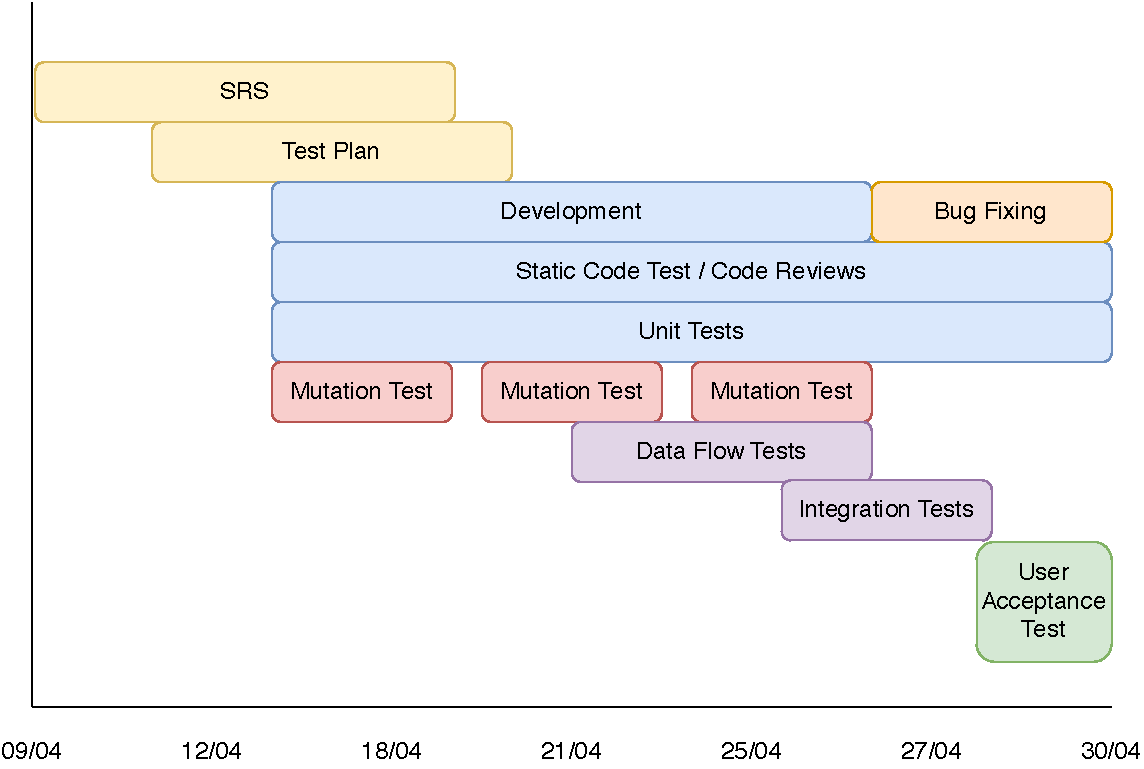
\includegraphics[scale=0.60]{ST_2019_Project_Test_Plan/figs/schedule.pdf}
    \caption{Schedule (approximately)}
    \label{fig:schedule}
\end{figure}

\begin{comment}
%%%%
% Objectives and Tasks
%%%%
\section{Objectives and Tasks}
\subsection{Objectives}
Describe the objectives supported by the Master Test Plan, For Example, defining tasks and responsibilities, a vehicle for communication, a document to be used as a service level agreement, etc.

\subsection{Tasks}
List all the tasks identified by this Test Plan, i.e., testing, post-testing, problem reporting, etc.

%%%%
% bla bla
%%%%
\section{bla bla}
\end{comment}


%%%%
% Development Environment
%%%%
\clearpage
\section{Development Environment}
This section gives a brief overview and insights about the development environment. Its purpose is to examine the circumstances and the environment under which the system (i.e. the programming code) is developed to ensure a flawless process pipeline and to provide a background for the actual test environment.

\subsection{Trunk-based Development Workflow}
\label{sec:trunk-workflow}
The development process is based on a mix between a Trunk-based and a Git(Hub) workflow. The combination of both creates a minimum of administration overhead and achieves a maximum of code quality.

The workflow consists of the \texttt{master} branch, which is open for every developer to push. But every feature, as well as every bugfix, is created in a separate \texttt{feature-branch}. After finishing the development of a specific branch, the branch is converted to a pull-request (PR). Another developer must review each PR. If and only if the reviewer marks the PR as approved, the PR is allowed to get merged into the master branch.

Through this code review strategy, i) a high \textbf{code quality} and ii) early \textbf{detection of bugs} is ensured, iii) \textbf{code-smells} are identified in an early stage, and iv) \textbf{knowledge sharing} among the developers is encouraged.

\begin{figure}[H]
\centering
    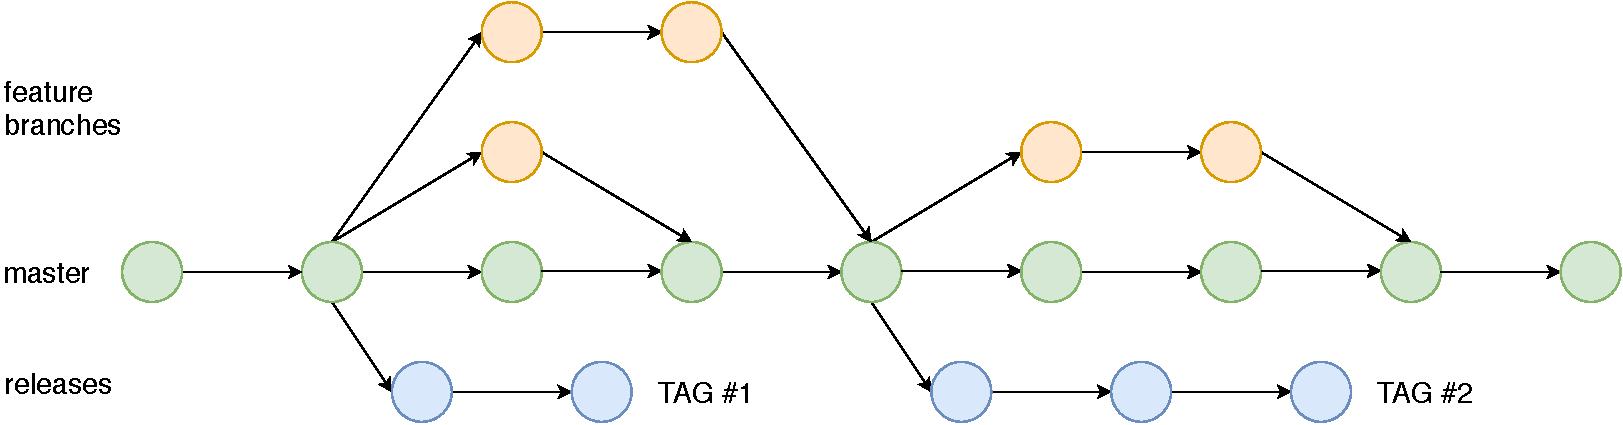
\includegraphics[scale=0.50]{ST_2019_Project_Test_Plan/figs/trunk_workflow.pdf}
    \caption{Trunk-based workflow}
    \label{fig:trunk-workflow}
\end{figure}


\subsection{Agile process with GitHub}
\label{sec:agile}
The project is structured in an iterative approach, focusing on continuous releases to gather feedback from every iteration. Since this project has no actual customer, the feedback comes from code reviews and continuous test iterations. One iteration phase contains 1) design, 2) development, 3) test, and 4) evaluation phase. To achieve agile project management, GitHub is used as distributed version control, source code management, and project management tool. The following subsections describe the various GitHub functions used.

\subsubsection{Projects}
As a central project management tool to organize and prioritize the different tasks, \textit{GitHub Projects} is used with an automated Kanban board configuration. Every issue and task is listed. The board represents the used workflow and gives an overview of all tasks, their status, and the assigned person. Figure \ref{fig:github-projects} shows an example of the configured Kanban board.

\begin{figure}[H]
\centering
    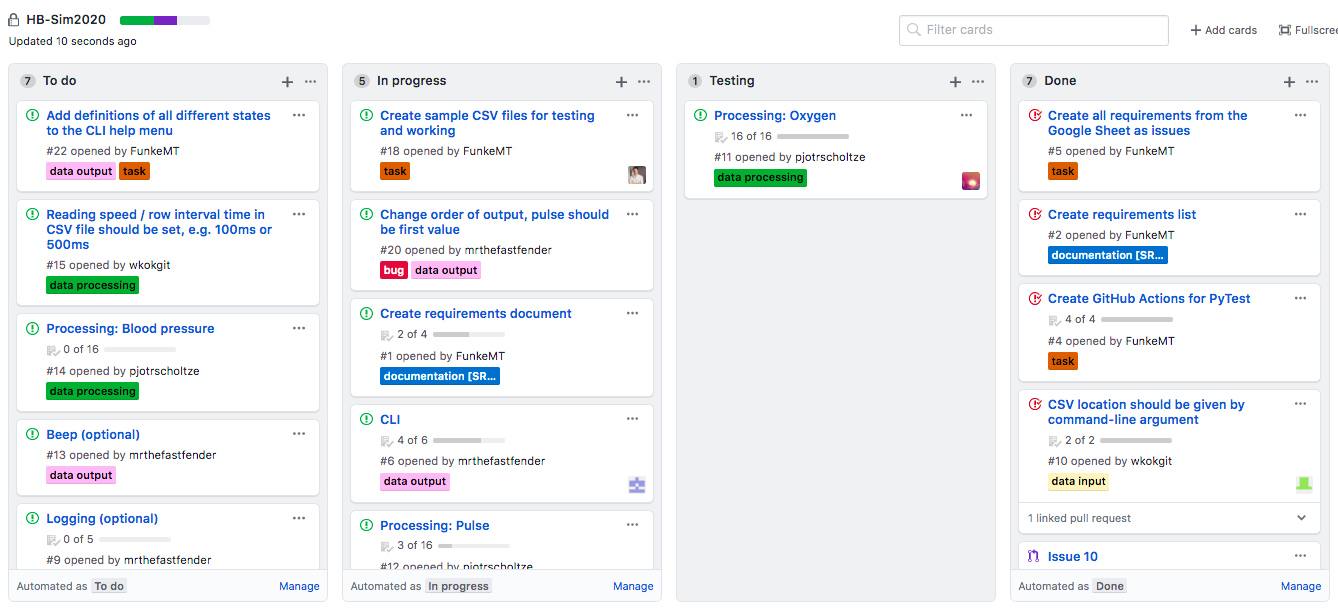
\includegraphics[scale=0.30]{ST_2019_Project_Test_Plan/figs/github_projects.png}
    \caption{GitHub Projects}
    \label{fig:github-projects}
\end{figure}

\subsubsection{Issues}
\label{sec:github-issues}
\textit{GitHub Issues} is used as a centralized bug-tracker and task management tool. Through different labels, management beyond source code issues and tasks are likely. GitHub allows issue referencing to commits. This allows tracking the feature and its assigned developer. Together with pull request reviewers, one feature/issue can be traced through its whole lifetime---from issue creation, development, review, testing, and integration. Figure \ref{fig:github-issues} shows an example issue list.

\begin{figure}[H]
\centering
    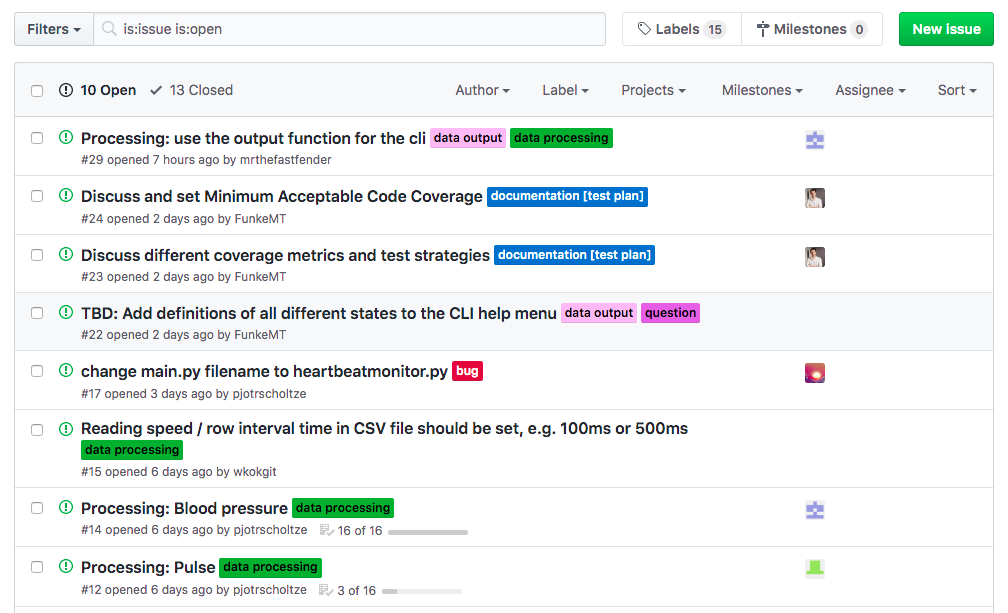
\includegraphics[scale=0.35]{ST_2019_Project_Test_Plan/figs/github_issues.png}
    \caption{GitHub Issues}
    \label{fig:github-issues}
\end{figure}

\subsubsection{Actions}
\label{sec:github-actions}
To automate several tasks, a \textit{GitHub Action} pipeline is installed. Along with every commit or merge into the master branch, the pipeline is triggered. The pipeline executes, among other things, the following tasks:

\begin{enumerate}
    \item Linter - run static code analysis
    \item PyTest - run unit tests
    \item PyTest Coverage - generate coverage report
\end{enumerate}

Figure \ref{fig:github-action} shows an extract of a successful build and its different actions. See section \ref{sec:test-strategy} for more details about static code analysis and unit tests.

\begin{figure}[H]
\centering
    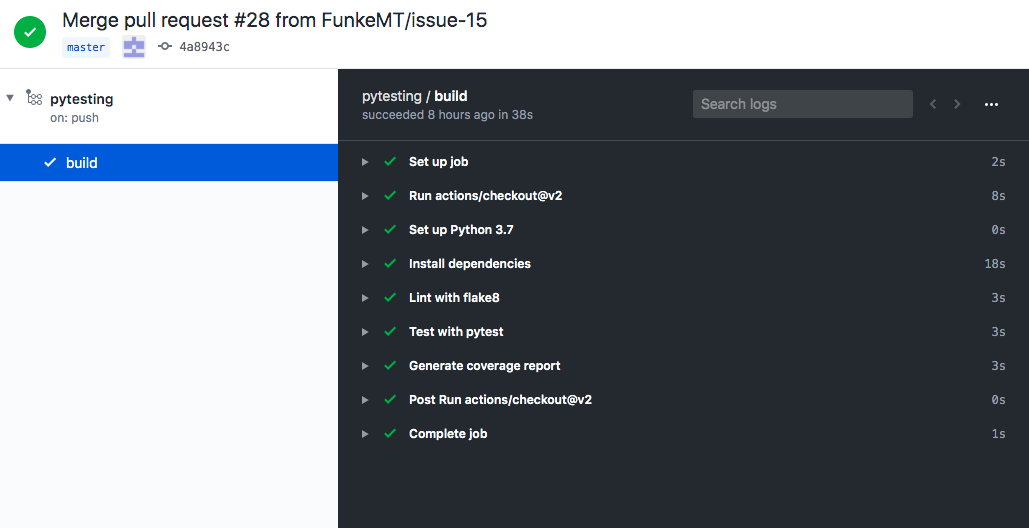
\includegraphics[scale=0.35]{ST_2019_Project_Test_Plan/figs/github_actions.png}
    \caption{GitHub Actions}
    \label{fig:github-action}
\end{figure}



\subsection{Code Style-guide}
The code development adhere to the "PEP 8 -- Style Guide for Python Code"\footnote{https://www.python.org/dev/peps/pep-0008/} and is fulfilled by using the Python code formatter \textit{Black}\footnote{https://github.com/psf/black} (version 19.10b0).


\subsection{Test-Driven Development}
\label{sec:tdd}
Together with agile project management (see section \ref{sec:agile}) we tried to approach the development in a test-driven method (TDD). The developers are obliged to write test functions consequently before the actual component is implemented. This ensures that only proven code is added which meets the specified requirements in the SRS. For more information about unit tests see section \ref{sec:unit-tests}.




%%%%
% Test Environment
%%%%
\clearpage
\section{Test Strategy} 
\label{sec:test-strategy}
\subsection{Code Review}
\subsubsection*{Purpose}
The usage of a random assignment to review code segments removes personal preferences between the developers, removes human bias, and helps to focus on technical facts.

\subsubsection*{Scope}
Code reviews should be applied on all system modules.

\subsubsection*{Method}
To achieve a random reviewer assignment to each developer, a small R-script is used (the R-script and its result after execution can be found in Appendix \ref{appendix:review-assignment}). The final assignment after the script execution is showed in table \ref{table:review-assignment}.


\subsubsection*{Testers}
\begin{table}[h]
{\renewcommand{\arraystretch}{\arraystrechlength}
    \begin{tabular}{ | m{100pt} | m{180pt} | }
    
    \hline
    \rowcolor{vu-blue}
    \textcolor{vu-white}{\textbf{Developer}} & \textcolor{vu-white}{\textbf{Gets Review From}} \\ \hline
    
    Sven Preng &
    Wouter Kok
    \\ \hline
    
    Pjotr Scholtze &
    Markus Funke
    \\ \hline
    
    Wouter Kok &
    Pjotr Scholtze
    \\ \hline
    
    Markus Funke &
    Sven Preng
    \\ \hline
    
    \end{tabular}
}
\caption{Review Assignment}
\label{table:review-assignment}
\end{table}


\subsubsection*{Test Acceptance}
The test strategy is a continuous strategy which will happen during the whole development phase. As in section \ref{sec:trunk-workflow} explained, each pull request has to pass a review strategy and is conducted by another developer. Every review is following these principles, which are based on\footnote{https://google.github.io/eng-practices/review/reviewer/}.

\begin{itemize}
    \item Is the code well structured?
    \item Is the functionality as in the SRS specified?
    \item Is the code as less complex as possible?
    \item Are the unit tests appropriate and designed well?
    \item Is the naming (methods, variables, etc.) well chosen?
    \item Do the comments explain \textit{why} instead of \textit{what} and are they clear formulated?
    \item Does the code follows the style guide?
\end{itemize}



 





\subsection{Static Code Analysis - linting}
\subsubsection*{Purpose}
As static code analysis the continuous development (CD) process should contain a static code analysis tool which is executed automatically and at code-compile time. The execution should be performed \textit{before} the unit tests. 

\subsubsection*{Scope}
Static code analysis should be applied on all system modules.

\subsubsection*{Method}
As in section \ref{sec:github-actions} already mentioned, the linting execution is performed by a GitHub Action through the Python library \textit{flake8}\footnote{https://flake8.pycqa.org/en/latest/} (version 3.7.9).

\subsubsection*{Testers}
All developers should keep an eye on the automatic reports generated by flake8 and integrate the results.

\subsubsection*{Test Acceptance}
The test strategy is a continuous strategy which will happen during the whole development phase.




\clearpage
\subsection{Unit Testing}
\label{sec:unit-tests}
To follow the TDD approach as described in section \ref{sec:tdd}, unit tests should be written and executed as in the workflow diagram (Figure \ref{fig:pytest-workflow}) described.

While we initially tried to follow the principles from TDD, we ended up using them sparsely. For the most part, the code was written before the tests were written.

\begin{figure}[H]
\centering
    
\includegraphics[scale=0.60]{ST_2019_Project_Test_Plan/figs/pytest_workflow.pdf}
    \caption{Unit Test Workflow}
    \label{fig:pytest-workflow}
\end{figure}


\subsubsection{PyTest}
\label{sec:pytest}
\subsubsection*{Purpose}
Unit testing is carried out throughout the entire implementation phase and starts from day one. Since TDD is chosen as a development process (see \ref{sec:tdd}), test cases should be written before the actual unit implementation. Omitting test cases leads to higher technical dept. Therefore test cases should be available for as many units as possible and as early as possible to save time in the actual integration phase and uncover bugs in an early stage.

\subsubsection*{Scope}
Unit testing should be applied to all system modules. Since the \textbf{data processing module} is the most important module (priority \textit{high}) it should get the most attention.

\subsubsection*{Method}
To write and execute unit tests, the Python extension \textit{PyTest}\footnote{https://docs.pytest.org/en/latest/} is used. The extension should be used on a local machine at development time. In addition, a GitHub Action (see section \ref{fig:github-action}) is executed to trigger PyTest automatically. To achieve an efficient test-case selection, such that all possible test instances are covered, \textbf{Equivalence Partitioning} (EP) and \textbf{Boundary Value Analysis} (BVA) are used.
\newline
\newline
As already mentioned, the data processing module is prioritized as \textit{high}. Hence, only for this module a dedicated spreadsheet with test-cases is prescribed. This spreadsheet has to be used by the developer to write the test cases for this modules. More test cases are acceptable, while less test cases are not acceptable. The other modules follows EP and BVA as well, but the developer has to decide which test-cases should be written to achieve the test acceptance. For those modules, the written test-cases itself serve as documentation. The spreadsheet for the data processing module can be found in Appendix \ref{appendix:bva}.


\subsubsection*{Testers}
All developers.

\subsubsection*{Test Acceptance}
see PyTest Coverage acceptance in \ref{sec:pytest-cov}.



\subsubsection{PyTest Coverage}
\label{sec:pytest-cov}
\subsubsection*{Purpose}
The purpose of test coverage is to find untested code segments and functions. It helps also to identify unnecessary test cases and uncovers paths in the application and code which are never be executed and meaningless. Together with the SRS, coverage reports identifies gaps in the requirements. The developer should not attempt to artificially increase test coverage, but should use the reports as information and identify vulnerabilities.

\subsubsection*{Scope}
Test coverage should be applied to all system modules. For modules with priority \textit{medium} or \textit{low} (e.g. UI), a lower test coverage is acceptable.

\subsubsection*{Method}
As major code coverage method \textbf{Statement Coverage} is used. The aim is that all executable statements in the code are executed at least once. 

The coverage report is created automatically by GitHub Actions (see section \ref{sec:github-actions}) and is based on the Python PyTest plugin \textit{PyTest-Cov}\footnote{https://pypi.org/project/pytest-cov/} (version 2.8.1). It is also possible to create the coverage report locally.



\subsubsection*{Testers}
All developers.

\subsubsection*{Test Acceptance}
Since the overarching system contains also of an user interface (printing to the CLI) which is prioritized in the SRS as \textit{Medium} and for which it is difficult to create reliable test cases, the test coverage acceptance is set to \textbf{96\%} (indicated by the blue dashed line in Figure \ref{fig:coverage}). To keep track of the coverage, Figure \ref{fig:coverage} examines the growth of the code statements in relation to the coverage in percentage (the diagram data are in appendix \ref{appendix:test-coverage-data}).

\begin{figure}[H]
\centering
    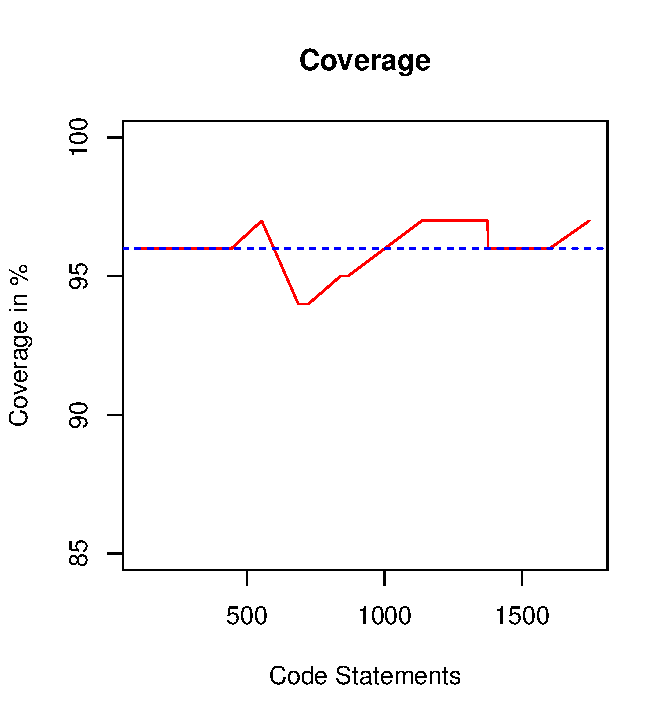
\includegraphics[scale=0.7]{ST_2019_Project_Test_Plan/figs/coverage.pdf}
    \caption{Statement Coverage Report, growth of code statement}
    \label{fig:coverage}
\end{figure}



\clearpage
\subsection{Mutation Testing}
\subsubsection*{Purpose}
Data processing includes the analysis of the incoming measurements (via CSV) and the classification of those values. This classifications (also known as status - see SRS for more information) could be life threatening in the worst case. To ensure a faultless behaviour and detect weaknesses in the tests and code, mutation tests are executed and analysed.

\subsubsection*{Scope}
Since the most important module is the \textbf{data processing module}, mutation tests should be executed only for this module.

\subsubsection*{Method}
To automate mutation testing with Python, \textit{mutmut}\footnote{https://mutmut.readthedocs.io/en/latest/} (version 2.0.0) is used. The workflow which should be stuck to for analyzing the processing module is explained in Figure \ref{fig:mutmut-workflow}.

\begin{figure}[H]
\centering
    
\includegraphics[scale=0.60]{ST_2019_Project_Test_Plan/figs/mutmut_workflow.pdf}
    \caption{Mutation Testing Workflow with \textit{mutmut}}
    \label{fig:mutmut-workflow}
\end{figure}

\subsubsection*{Testers}
Developers who are involved in the data process implementation.

\subsubsection*{Test Acceptance}
The Mutation Score (MS) is calculated as $MS = \frac{\#killed mutants}{total} \cdot 100 [\%]$ and should be at least $70\%$ or higher in the final release. The focus should be rather on the report analyzing process and find weaknesses than increasing the MS artificially. A protocol for the different milestones and test-phases are provided in table \ref{table:mutmut-protocol}. Since the execution of the mutation tests itself and the analyzing process costs a lot of time, mutation tests should be not automated (i.e. GitHub Actions - see section \ref{sec:github-actions}).

\clearpage
\begin{longtable}[l]{ | m{50pt} | m{50pt} | m{80pt} | m{40pt} |  m{140pt} | }

    \rowcolor{vu-blue}
    \textcolor{vu-white}{\textbf{Version}} &
    \textcolor{vu-white}{\textbf{Date}} &
    \textcolor{vu-white}{\textbf{Developer}} &
    \textcolor{vu-white}{\textbf{MS [\%]}} &
    \textcolor{vu-white}{\textbf{\textit{mutmut} Result}} \\ \hline
    
    v0.5 &
    2020-04-19 &
    Markus Funke &
    61 \% &
    \begin{itemize}
        \item killed: 33
        \item timeout: 0
        \item suspicious: 0
        \item survived: 21
        \item skipped: 0
    \end{itemize} \\ \hline
    
    v0.6 &
    2020-04-21 &
    Markus Funke &
    64 \% &
    \begin{itemize}
        \item killed: 55
        \item timeout: 0
        \item suspicious: 0
        \item survived: 31
        \item skipped: 0
    \end{itemize} \\ \hline
    
    v0.9 &
    2020-04-25 &
    Pjotr Scholtze &
    100 \% &
    \begin{itemize}
        \item killed: 87
        \item timeout: 0
        \item suspicious: 0
        \item survived: 0
        \item skipped: 0
    \end{itemize} \\ \hline
    
    \caption{Mutation Test Protocol}
    \label{table:mutmut-protocol}
    \\

\end{longtable}



\clearpage
\section{Data Flow Diagram}
\subsubsection*{Purpose}
The Data Flow visualizes how information flows throughout our system. Thus brings a better view of the system and makes it easier to see data changes and which data should be tested for validity.   
\subsubsection*{Scope}
The scope of the data flow is mostly within the \textit{Data processing} module in which it processes user input data. After processing the data can be used to output.
\subsubsection*{Method}
A Data Flow is created which is shown in Figure \ref{fig:dataflow}. 
\begin{figure}[H]
    \centering
    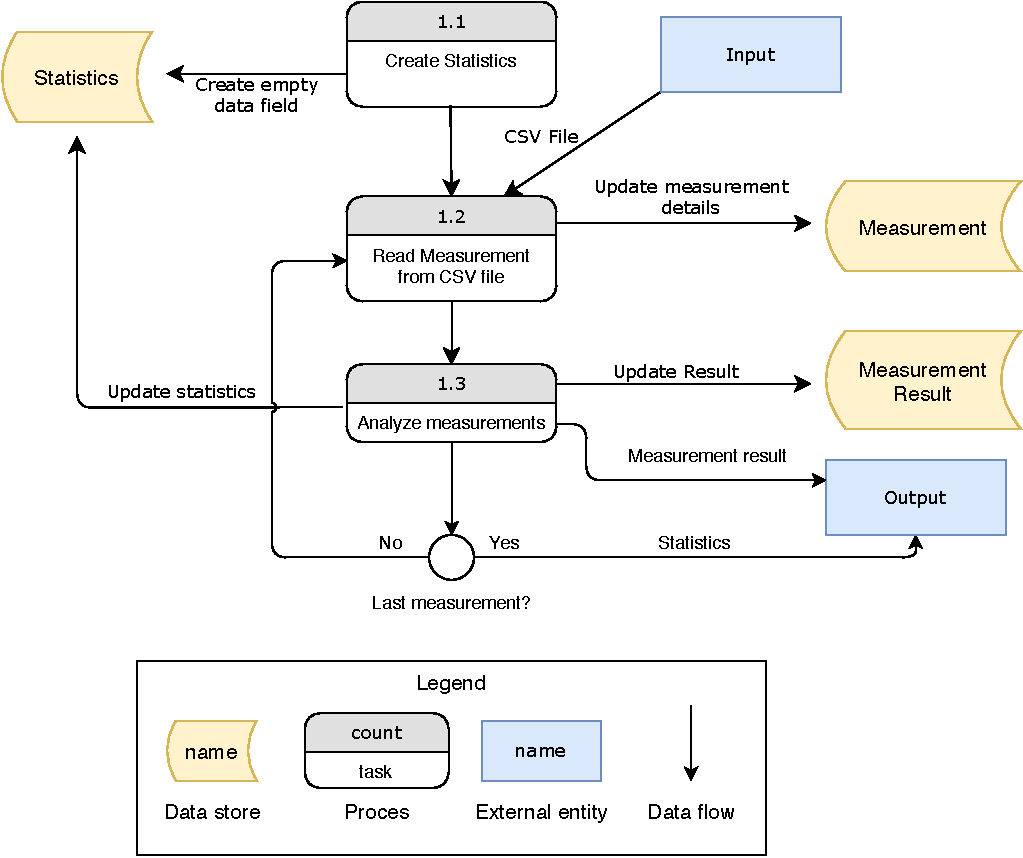
\includegraphics[scale=0.70]{ST_2019_Project_Test_Plan/figs/Data_Flow_Diagram.pdf}
    \caption{Data Flow Diagram}
    \label{fig:dataflow}
\end{figure}
\subsubsection*{Testers}
Developers who are involved in the data process implementation.
\subsubsection*{Test Acceptance}
Only if every data flow path in Figure \ref{fig:dataflow} is tested with all CSV files, the test may be accepted.

We used various CSV values with injected issues to test the program. We covered these issues:
\begin{itemize}
    \item Missing headers
    \item Malformed headers
    \item Too many headers
    \item String input instead of numeric input
    \item Numeric input outside boundary
    \item Integer overflow input
    \item Missing values in a recording row
    \item With only headers and no values
\end{itemize}


\clearpage
\section{Integration Test}
\subsubsection*{Purpose}
Integrate all different software modules into one logically group to test it as a single system to identify and uncover interaction problems between these modules.

\subsubsection*{Scope}
All different modules as in the SRS and in \ref{table:func-groups} defined. Module i) data input, ii) data processing, and iii) data output will be grouped into the final system \textit{HB-Sim2020}.

\subsubsection*{Method}
To integrate all modules into the actual HB-Sim2020 system, a top-down approach should be used. In particular, first (1) combine module \textit{data input} and \textit{data processing}. In the second step (2) the module \textit{data output} is integrated. This approach ensures that data input and data ouput works correctly together---independently from the data output layer.

\begin{figure}[H]
\centering
    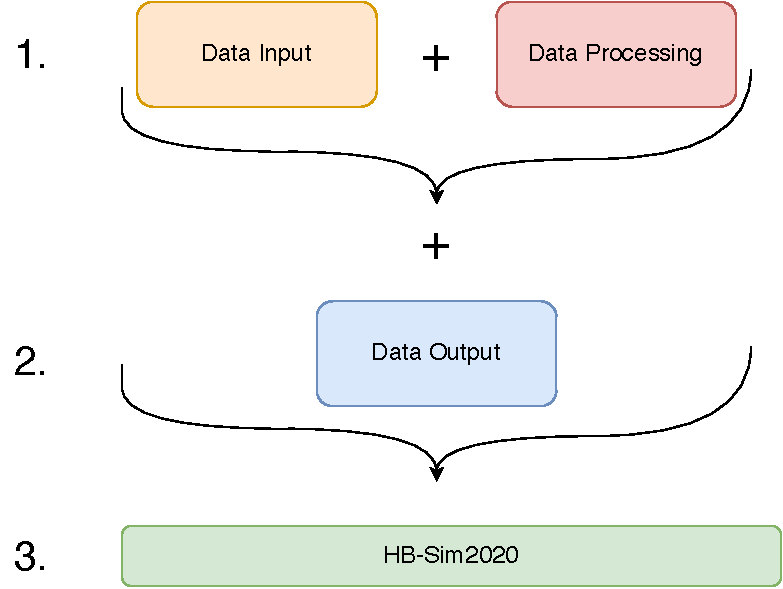
\includegraphics[scale=0.60]{ST_2019_Project_Test_Plan/figs/integration.pdf}
    \caption{Module Integration}
    \label{fig:integration}
\end{figure}


\subsubsection*{Testers}
All developers.

\subsubsection*{Test Acceptance}
Test should be performed according to the SRS. The following table gives an overview of the requirements which have to be \textbf{tested} and have to be \textbf{fulfilled} according to each integration phase.

\clearpage
\begin{longtable}[l]{ | m{55pt} | m{55pt} | m{250pt} | }

    \rowcolor{vu-blue}
    \textcolor{vu-white}{\textbf{Integration Phase}} &
    \textcolor{vu-white}{\textbf{Modules}} &
    \textcolor{vu-white}{\textbf{Requirements}} \\ \hline
    
    1 &
    Data Input \& Data Processing &
    \begin{itemize}
        \item SR-\#4.2.1: Input recording location
        \item SR-\#4.2.2: Comma-separated values (CSV) file
        \item SR-\#4.2.3: Oxygen measurements
        \item SR-\#4.2.4: Pulse measurements
        \item SR-\#4.2.5: Blood pressure measurements
    \end{itemize} \\ \hline
    
    2 &
    Data Output &
    \begin{itemize}
        \item Requirements from phase \#1 plus:
        \item SR-\#4.2.6: Data output - statistic
        \item SR-\#4.2.7: User interface
        \item SR-\#4.2.8: Logging
    \end{itemize} \\ \hline
    
    3 &
    HB-Sim2020 &
    \begin{itemize}
        \item Requirements from phase \#1 plus
        \item Requirements from phase \#2.
    \end{itemize} \\ \hline
    
    General &
    General &
    For all test executions, all testing CSV files have to be used and executes before the test will be accepted and the next integration phase can be started. Repository paths to CSV testing files:
     \begin{itemize}
        \item \texttt{heartmonitor/input/normal\_100.csv}
        \item \texttt{heartmonitor/input/normal\_with\_errors\_100.csv}  
        \item \texttt{heartmonitor/input/random\_100.csv} 
        \item \texttt{heartmonitor/input/simulation.csv}
    \end{itemize}
    \\ \hline
    

    \caption{Integration Test Strategy}
    \label{table:integrationtest}
    \\

\end{longtable}





\clearpage
\section{User Acceptance Test}
\subsubsection*{Purpose}
After fully developing the software of this project, a user acceptance test is done as a final step towards rolling out the application. This test is done after various levels of testing are already completed and aimed at usefulness and usability instead of cohering to requirements. The goal is to see if the customer's needs are solved.
\subsubsection*{Scope}
The scope is the whole final application. 
\subsubsection*{Method}
There are User Acceptance Testing Test Cases created to show the steps a tester has to do to fulfill the user's needs.

\begin{table}[H]
{
\begin{tabular}{ | >{\columncolor{vu-blue}\color{vu-white}}m{100pt} |  m{238pt} | } 
\hline
User Story              & As a doctor I want to be able to easily start-up the system  \\ 
\hline
Test Scenario Steps     & 
\begin{enumerate}
    \item Open a command-line interface
    \item Make sure \textbf{HB-Sim2020.exe} and \textbf{simulations.csv} are in the same folder
    \item Go to the folder holding both files
    \item Run: \textbf{python HB-Sim2020.exe --path simulation.csv} 
\end{enumerate}  \\ 
\hline
\end{tabular}
}
\caption{UAT TC1: Start-up the system}
\label{table:TC1}
\end{table}

\begin{table}[H]
{
\begin{tabular}{ | >{\columncolor{vu-blue}\color{vu-white}}m{100pt} |  p{238pt} | } 
\hline
User Story              & As a doctor I want to be able to see my patients oxygen, pulse and blood pressure levels.  \\ 
\hline
Test Scenario Steps     & 
\begin{enumerate}
    \item Make sure the system is started
    \item Look at the incoming measurement results coming in every second in the CLI
    \item Execute actions upon those results
\end{enumerate}  \\ 
\hline
\end{tabular}
}
\caption{UAT TC2: Use heartbeat monitor as intended}
\label{table:TC2}
\end{table}

\begin{table}[H]
{
\begin{tabular}{ | >{\columncolor{vu-blue}\color{vu-white}}m{100pt} |  p{238pt} | } 
\hline
User Story              & As a doctor I want to be able to see the statistics of what happened during the last run.  \\ 
\hline
Test Scenario Steps     & 
\begin{enumerate}
    \item Make sure the system is started
    \item Exit the program by using CTRL-C
    \item Look at the statistics given from the system's run
\end{enumerate}  \\ 
\hline
\end{tabular}
}
\caption{UAT TC3: See statistics}
\label{table:TC3}
\end{table}

\subsubsection*{Testers}
For the reason that we're doing this project for the Software Testing course, we're unable to let real doctors, which would be the end-users/client, test our project. Therefore we have chosen that we ourselves do this test, keeping in mind that it is not the right way to do it.
\subsubsection*{Test Acceptance}
The tests are executed and if there are any faults, they are being noted and fixed by the development team.



\clearpage
%%%%
% Test Environment
%%%%
\section{Test Environment}
If no specific test method is specified in section Test Strategy \ref{sec:test-strategy} (e.g. GitHub Actions), the tests have to be done at a local development environment. The following different hard-/software combinations are available and admitted.

\subsection{Linux}
\begin{itemize}
    \item OS Version: Ubuntu 20.04 LTS
    \item Terminal: XFCE 4 Terminal with ZSH
\end{itemize}

\subsection{MacOS}
\begin{itemize}
    \item OS Version: MacOS 10.13.6
    \item Terminal: iTerm2
\end{itemize}

\subsection{Windows}
\begin{itemize}
    \item OS Version: Windows 10.0.18363 Build 18363
    \item Terminal: CMD
\end{itemize}

\subsection{Windows}
\begin{itemize}
    \item OS Version: WSL subsystem version 4.4.0-18362-Microsoft x86\_64
    \item Terminal: bash
\end{itemize}


\clearpage
%%%%
% Appendix
%%%%
\section{Appendix}

\subsection{Code Review Assignment}
\label{appendix:review-assignment}
\begin{lstlisting}[language=R, caption=Random Mapping - R Code, captionpos=b]
students = c("Sven", "Pjotr", "Wouter", "Markus")
test_assign = data.frame(
    "Student" = students,
    "getsReviewFrom" = sample(students)
)
print(test_assign)
\end{lstlisting}

\begin{figure}[H]
\centering
    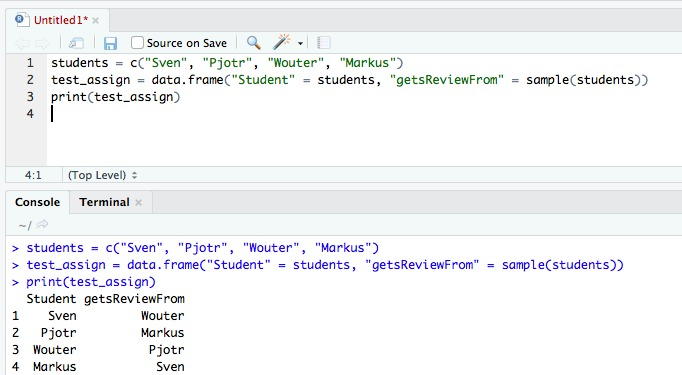
\includegraphics[scale=0.50]{figs/r-code.jpeg}
    \caption{Random Mapping - Result}
    \label{fig:mapping-result}
\end{figure}


\clearpage
\subsection{Test Coverage Data}
\label{appendix:test-coverage-data}
\begin{lstlisting}[caption=Test coverage data, captionpos=b]
statements,miss,coverage
115,6,96
227,9,96
251,9,96
322,12,96
324,13,96
444,13,96
554,16,97
687,44,94
690,44,94
716,44,94
724,44,94
840,43,95
867,43,95
1136,39,97
1153,40,97
1375,48,97
1377,50,96
1601,63,96
1745,57,97
\end{lstlisting}

\clearpage
\subsection{Data Processing Module - BVA and EP}
\label{appendix:bva}
Test overview for Equivalence Partitioning and Boundary Value Analysis testing techniques. Intervals are given as mathematical intervals (see \footnote{https://en.wikipedia.org/wiki/Interval\_(mathematics)}).

\begin{figure}[H]
\centering
    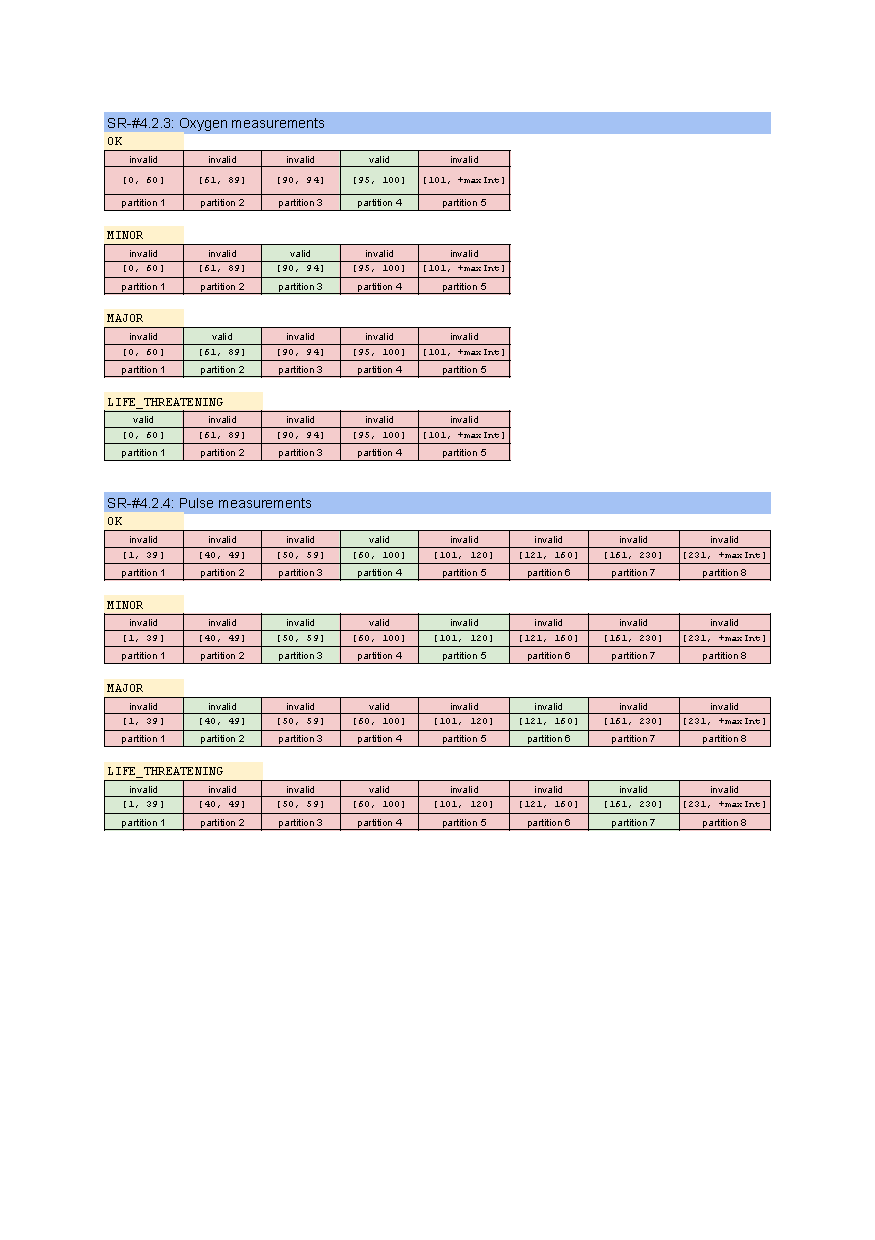
\includegraphics[scale=0.8, page=1]{ST_2019_Project_Test_Plan/figs/DataProcessingModuleTest.pdf}
\end{figure}
\begin{figure}[H]
\centering
    \includegraphics[scale=0.9, page=2]{ST_2019_Project_Test_Plan/figs/DataProcessingModuleTest.pdf}
\end{figure}







\begin{comment}
\clearpage
\section{Tables}
All tables are colored by the VU corporate identity colors. See preamble section \texttt{VU colors}.

\subsection{Example \#1}
\begin{table}[h]
{\renewcommand{\arraystretch}{\arraystrechlength}
    \begin{tabular}{ | >{\columncolor{vu-grey-50}}m{100pt} | m{230pt} | }
    
    \hline
    \rowcolor{vu-blue}
    \textcolor{vu-white}{\textbf{Headline 1}} & \textcolor{vu-white}{\textbf{Headline 2}} \\ \hline
    
    Example &
    My cell example
    \\ \hline
    
    Example &
    Lorem ipsum
    \\ \hline
    
    \end{tabular}
}
\end{table}


\subsection{Example \#2}
\begin{table}[h]
{\renewcommand{\arraystretch}{\arraystrechlength}
    \begin{tabular}{ | >{\columncolor{vu-blue}\color{vu-white}}m{100pt} | m{230pt} | }
    \hline
    
    \textbf{Example} &
    Lorem ipsum
    \\ \hline
    
    \textbf{Example} &
    Lorem ipsum
    \\ \hline
    
    \textbf{Example} &
    Lorem ipsum
    \\ \hline
    
    \end{tabular}
}
\end{table}


\subsection{Example \#3}
\begin{table}[h]
{\renewcommand{\arraystretch}{\arraystrechlength}
\begin{tabular}{ | >{\columncolor{vu-blue}\color{vu-white}}m{70pt} | >{\columncolor{vu-grey-50}}m{330pt} | } 
\hline
Example                  & \textbf{Con\#1}: Example \\ 
\hline
Example         & \makecell*[l]{\textbf{Cr\#1}: Example \\ \textbf{Cr\#2}: Example}  \\
\hline
\end{tabular}
}
\end{table}


\subsection{Example \#4}
\begin{table}[H]
{\renewcommand{\arraystretch}{\arraystrechlength}
\begin{tabular}{ | >{\columncolor{vu-blue}\color{vu-white}}m{70pt} | >{\columncolor{vu-grey-50}}m{80pt} | p{238pt} | } 
\hline
Option 1                  & Example & \textbf{Example}: Lorem Ipsum  \\ 
\hline
                          & Example   & Lorem ipsum dolor sit amet, consetetur sadipscing elitr, sed diam nonumy eirmod tempor invidunt ut labore et dolore magna aliquyam erat, sed diam voluptua. At vero eos et accusam et justo duo dolores et ea rebum. Stet clita kasd gu                   \\ 
\hline
                          & Example  & Example.                        \\ 
\hline
                          & Example  & \makecell*[{{p{238pt}}}]{
                          Lorem \\ \\
                          Ipsum
                          }\\ 

\hline
\end{tabular}
}
\end{table}


\clearpage
\begin{thebibliography}{00}
\bibitem{google-review}Google Inc., \textit{How to do a code review}, eng-practices, 2020. [Online]. Available: https://google.github.io/eng-practices/review/reviewer/. [Accessed: 27- Apr- 2020].
\end{thebibliography}
\end{comment}


\end{document}
